\chapter[%
    Linear-Response Density Cumulant Theory for Excited States:\\
	Better Algorithms, Bigger Systems
]{%
    Linear-Response Density Cumulant Theory for Excited States:\\
	Better Algorithms, Bigger Systems
}
\label{ch:davidson}


\begin{figure}[h!]
    \centering
    \caption{%
        \label{fig:davidson}
        A schematic illustrating the sequence of reduced representations of
        \(\mathbf{E}\) in the algorithm employed in this study.
        The colored entries must be explicitly computed, whereas the gray
        entries are determined by Hermitian symmetry.
    }
    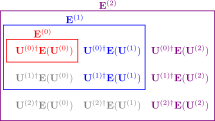
\includegraphics[width=8.5cm]{figures/davidson.pdf}
\end{figure}

We have implemented the LR-ODC-12 method using a multi-root Davidson algorithm,
which solves the linear-response generalized eigenvalue problem by progressively
growing an expansion space for the \(n_\mathrm{root}\) lowest generalized
eigenvectors of \(\mathbf{E}\) and \(\mathbf{M}\).
The general procedure looks as follows:
\begin{enumerate}
    \item
        \label{item:davidson-initialization}
        Initialize the expansion space with a set of \(n_\mathrm{guess}\geq
        n_\mathrm{root}\) orthonormal vectors.
        \[
            \mathbf{R}^{(0)}
            =
            (
                \mathbf{u}_1^{(0)}
                \cdots
                \mathbf{u}_{n_\mathrm{guess}}^{(0)}
            )
        \]
    \item
        \label{item:davidson-step-one}
        Express the energy-Hessian and metric matrices in the reduced expansion
        space.
        \[
            \mathbf{E}^{(i)}
            =
            \mathbf{R}^{(i)\dagger}
            \mathbf{E}(\mathbf{R}^{(i)})
        \]
        \[
            \mathbf{M}^{(i)}
            =
            \mathbf{R}^{(i)\dagger}
            \mathbf{M}(\mathbf{R}^{(i)})
        \]
    \item
        Solve for the \(n_\mathrm{root}\) highest eigenvectors of the
        inverse eigenvalue equation.
        \[
            \mathbf{M}^{(i)}
            \mathbf{z}_k^{(i)}
            =
            \mathbf{E}^{(i)}
            \mathbf{z}_k^{(i)}/
            \omega_k^{(i)}
        \]
    \item
        Determine the residual for each root.
        \[
            \mathbf{d}_k^{(i)}
            =
            \mathbf{M}(\mathbf{z}_k^{(i)})
            -
            \mathbf{E}(\mathbf{z}_k^{(i)})/
            \omega_k^{(i)}
        \]
        If the residual elements are sufficiently small we consider the
        eigenvectors converged and exit the loop.
    \item
        \label{item:davidson-step-three}
        Form new direction vectors by preconditioning the residuals.
        \[
            \mathbf{g}_k^{(i+1)}
            =
            -
            (
                \tilde{\mathbf{M}}
                -
                \tilde{\mathbf{E}}/
                \omega_k^{(i)}
            )^{-1}
            \mathbf{d}_k
        \]
        The tildes in this equation denote diagonal approximations to these
        matrices.
    \item
        Project out the span of the current expansion space from the new
        direction vectors.
        \[
            \mathbf{J}^{(i+1)}
            =
            (\mathbf{1} - \mathbf{R}^{(i)}\mathbf{R}^{(i)\dagger})
            (\mathbf{g}_1^{(i+1)}\cdots \mathbf{g}_{n_\mathrm{root}}^{(i+1)})
        \]
    \item
        Determine an orthonormal basis for the new direction vectors using a
        compressed singular value decomposition, and add these new vectors to
        the expansion space.
        \[
            \mathbf{J}^{(i+1)}
            \approx
            \mathbf{U}^{(i+1)}
            \boldsymbol\Sigma^{(i+1)}
            \mathbf{V}^{(i+1)\dagger}
        \]
        \[
            \mathbf{R}^{(i+1)}
            \leftarrow
            (\mathbf{R}^{(i)}\ \mathbf{U}^{(i+1)})
        \]
    \item
        Increment \(i\) and return to step~\ref{item:davidson-step-one}.
\end{enumerate}
A key feature of this algorithm is that we never need to explicilty construct
the energy-Hessian and metric matrices in memory, only their images over the
expansion space.

For the diagonal approximations in step~\ref{item:davidson-step-three} we use
the following.
\[
    \tilde{\mathbf{S}}_{11}
    \equiv
    \mathbf{1}_1
\]
\[
    (\tilde{\mathbf{A}}_{11})_{ia,ia}
    \equiv
    -
    f_i^i
    +
    f_a^a
\]
\[
    (\tilde{\mathbf{A}}_{22})_{ijab,ijab}
    \equiv
    -
    \mathcal{F}_i^i
    -
    \mathcal{F}_j^j
    -
    \mathcal{F}_a^a
    -
    \mathcal{F}_b^b
\]
These can also be used to construct the initial expansion space in
step~\ref{item:davidson-initialization}, namely by including unit vectors for
the \(n_\mathrm{guess}\) smallest positive entries in \(\tilde{\mathbf{E}}\).


\subsection{Ethylene, Butadiene, and Hexatriene}
\label{sec:alkenes}

\begin{table*}[h!]
    \centering
    \caption{%
        \label{tab:alkenes}
        Vertical excitation energies computed using LR-OLCCD, LR-ODC-12, and
        EOM-CCSD for the low-lying electronic states of ethylene (\ce{C2H4}),
        butadiene (\ce{C4H6}), and hexatriene (\ce{C6H8}).
        Computations employed the ANO-L-pVDZ (for \ce{C4H6} and \ce{C6H8}) and
        ANO-L-pVTZ (for \ce{C2H4}) basis sets and the MP2/cc-pVQZ optimized
        geometries.
        For LR-OLCCD and LR-ODC-12, oscillator strengths of the allowed
        transitions are given in parentheses.
        All electrons were correlated in all computations.
        Also shown are the excitation energies from the frozen-core
        semistochastic heat-bath CI (SHCI) method, extrapolated to full CI
        limit.
    }
    \begin{threeparttable}
        \begin{tabular}{clccccc}
            \hline
            \hline
            && EOM-CCSD & LR-OLCCD & LR-ODC-12 & SHCI\tnote{a} \\
            \hline
            \ce{C2H4}
            &
            \({}^3\mathrm{B_{1u}}\) &
            4.46 & 4.66 & 4.52 & 4.59 \\ 
            &
            \({}^1\mathrm{B_{1u}}\) &
            8.14 & 8.20 (1.8) & 8.14 (1.9) & 8.05
            \\
            \hline                           
            \ce{C4H6}                        
            &
            \({}^3\mathrm{B_{u}}\) &
            3.20 & 3.58 & 3.43 & 3.37 \\
            &
            \({}^1\mathrm{B_{u}}\) &
            6.53 & 6.76 (4.2) & 6.67 (4.4) & 6.45 \\
            &
            \({}^1\mathrm{A_{g}}\) &
            7.28 & 7.14 & 6.81 & 6.58
            \\
            \hline                           
            \ce{C6H8}
            &
            \({}^3\mathrm{B_{u}}\) &
            2.64 & 3.01 & 2.83 & 2.77 \\
            &
            \({}^1\mathrm{B_{u}}\) &
            5.60 & 5.89 (6.5) & 5.74 (8.1) & 5.59 \\
            &
            \({}^1\mathrm{A_{g}}\) &
            6.55 & & 5.73 & 5.58 \\
            \hline
            \hline
        \end{tabular}
        \begin{tablenotes}
            \item[a]
                The SHCI computations used the same basis sets and optimized
                geometries as those used for LR-OLCCD, LR-ODC-12, and EOM-CCSD.
        \end{tablenotes}    
    \end{threeparttable}
\end{table*}
